\documentclass{exam}
\usepackage{mycommands,amsmath,amsfonts,tikz,xeCJK}
\setCJKmainfont{STSong}

\begin{document}
\begin{questions}
\question
设$z=\gamma(t)$($a\le t\le b$)是一条可求长曲线,$f$是定义在$\gamma$上的函数,
沿$\gamma$的正方向取分点\[\gamma(a)=z_0,z_1,z_2,\cdots,z_n=\gamma(b),\]
在$\gamma$中从$z_{k-1}$到$z_k$的弧段上任取点$\zeta_k$, $k=1,\cdots,n$,作Riemann和
\begin{equation}\label{eq3.1.1}
  \sum_{k=1}^n f(\zeta_k) (z_k - z_{k-1}).
\end{equation}

用$s_k$记弧段$z_{k-1}z_k$的长度,如果当$\lambda=\max\{s_k:1\le k\le n\}\to0$时,不论$\zeta_k$的取法如何,和式 \eqref{eq3.1.1} 总有一确定的极限,就称此极限为$f$沿
$\gamma$的积分,记为$\int\limits_\gamma f(z)\diff z$,即
\[
  \int\limits_\gamma f(z)\diff z = \lim_{\lambda\to0}\sum_{k=1}^nf(\zeta_k)(z_k-z_{k-1}).
\]
\begin{figure}[!ht]
%   \centering
\flushleft
  \begin{tikzpicture}
    \draw(-4,0)node[below]{$z_0=\gamma(a)$}arc(180:90:4)node[right]{$z_n=\gamma(b)$};
    \foreach \x in {180,170,155,140,130,125,120,105,90}
      \fill(\x:4)circle(1pt);
    \draw(170:4)node[left]{$z_1$}(130:4)node[above left]{$z_{k-1}$}
         (125:4)node[below right]{$\zeta_k$}(120:4)node[above left]{$z_k$};
  \end{tikzpicture}
%   \caption{\label{fig3.1}}
\end{figure}

\question
计算积分$\int\limits_\gamma\frac{\diff z}{(z-a)^n}$,这里,$n$是任意整数,
$\gamma$是以$a$为中心、以$r$为半径的圆周.

\newpage

\question
如果$\gamma$的长度为$L,M=\sup_{z\in\gamma}|f(z)|$,那么
\begin{equation}\label{eq3.1.4}
  \bigg|\int\limits_\gamma f(z)\diff z\bigg|\le ML.
\end{equation}

\question
证明$|\int _Ce^{iz}\diff z|<\pi$, 其中C为上半圆周,从$R$到$-R$.
\vspace*{1in}

\question
设$D=\{z\in\mathbb{C}:\theta_0<\operatorname{arg}(z-a)<\theta_0+\alpha\}$($0<\alpha\le2\pi$),$f$在$\bar D\backslash\{a\}$上连续. 证明:
\begin{parts}
  \part 如果$\lim_{\substack{z\to a\\z\in\bar D\backslash\{a\}}}(z-a)f(z)=A$,那么
    \[
      \lim_{r\to0}\int\limits_{\substack{|z-a| = r\\z\in\bar D}}f(z)\diff z = i\alpha A;
    \]
  \part 如果$\lim_{\substack{z\to \infty\\z\in\bar D\backslash\{a\}}}(z-a)f(z)=B$,那么
    \[
      \lim_{R\to\infty}\int\limits_{\substack{|z-a|=R\\z\in \bar D}}f(z)\diff z = i\alpha B.
    \]
\end{parts}

\newpage

\question
\begin{parts}
\part 计算积分 $\int\limits_\gamma\frac{2z-3}z\diff z$,其中,$\gamma$为
    \begin{subparts}
      \subpart 沿圆周 $\{z:|z|=2\}$ 的上半圆,从 $-2$ 到 $2$;
      \subpart 沿圆周 $\{z:|z|=2\}$ 的下半圆,从 $-2$ 到 $2$;
      \subpart 沿圆周 $\{z:|z|=2\}$ 的正向.
    \end{subparts}
\part 计算积分 $\int\limits_{|z|=1}\frac{\diff z}{z+2}$,并证明:
    \[
      \int_0^\pi\frac{1+2\cos\theta}{5+4\cos\theta} \diff\theta = 0.
    \]
\part 计算积分 $\int\limits_{|z|=3}\frac{2z-1}{z(z-1)}\diff z$.
\end{parts}

\newpage

\question
\begin{parts}
    \part
    设$D$是$\mathbb{C}$中的单连通域,如果$f\in H(D)$,那么对$D$中任意的可求长闭曲线$\gamma$,均有
\[\int\limits_\gamma f(z)\diff z=0.\]
\part
设$D$是可求长简单闭曲线$\gamma$的内部,若$f\in H(D)\cap C(\bar D)$,则
  \[
    \int\limits_\gamma f(z)\diff z= 0.
  \]
  \part
  设$\gamma_0,\gamma_1,\cdots,\gamma_n$是$n+1$条可求长简单闭曲线,$\gamma_1,\cdots,\gamma_n$都在$\gamma_0$的内部,$\gamma_1,\cdots,\gamma_n$中的每一条都在其他$n-1$条的外部,$D$是由这$n+1$条曲线围成的域,用$\gamma$记$D$的边界.如果$f\in H(D)\cap C(\bar D)$,那么
  \begin{equation}\label{eq3.2.4}
    \int\limits_\gamma f(z)\diff z = 0,
  \end{equation}
  这里,积分沿$\gamma$的正方向进行. \eqref{eq3.2.4} 式也可写为
  \begin{equation}\label{eq3.2.5}
    \int\limits_{\gamma_0}f(z)\diff z=\int\limits_{\gamma_1}f(z)\diff z +
    \cdots+\int\limits_{\gamma_n}f(z)\diff z,
  \end{equation}
  \eqref{eq3.2.5} 式右端的积分分别沿$\gamma_1,\cdots,\gamma_n$的逆时针方向进行.
\end{parts}
\begin{minipage}{0.35\textwidth}
    \centering
    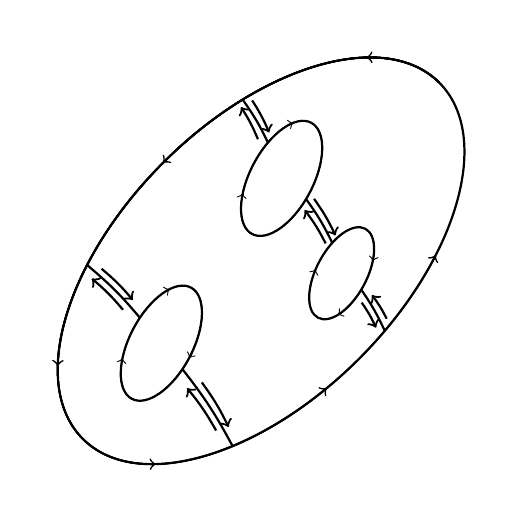
\begin{tikzpicture}[thick,rotate=45,scale=0.8]
      \draw(0,0)ellipse(4 and 2.2);
      \foreach \x in {30,90,150,210,260,300.360}
        \draw[->,semithick](4,0)arc(0:\x: 4 and 2.2);
        \draw[rotate around={17:(-1,0.2)}](-1,0.5)arc(0:360:1 and 0.5);
      \foreach \x in {-90,-240,-325}
        \draw[rotate around={17:(-1,0.2)},->,thin](-1,0.5)arc(0:\x: 1 and 0.5);
      \begin{scope}[shift={(3.2,0.5)}]
        \draw[rotate around={17:(-1,0.2)}](-1,0.5)arc(0:360:1 and 0.5);
        \foreach \x in {-240,-330}
          \draw[rotate around={17:(-1,0.2)},->,thin](-1,0.5)arc(0:\x: 1 and 0.5);
      \end{scope}
      \begin{scope}[shift={(2.4,-1.2)},scale=0.8]
        \draw[rotate around={17:(-1,0.2)}](-1,0.5)arc(0:360:1 and 0.5);
        \foreach \x in {-60,-140,-260}
          \draw[rotate around={17:(-1,0.2)},->,thin](-1,0.5)arc(0:\x: 1 and 0.5);
      \end{scope}
  
      \draw(-2,0.72)[bend right=5]to(-2,1.9);
      \draw[->](-2.1,1)[bend right=5]to(-2.1,1.7);
      \draw[->](-1.88,1.7)[bend left=5]to(-1.88,1);
  
      \draw(1.4,1.24)[bend right=5]to(1.6,2);
      \draw[->](1.33,1.4)[bend right=5]to(1.5,1.95);
      \draw[->](1.7,1.9)[bend left=5]to(1.53,1.35);
  
      \draw(-2.1,-0.34)[bend left=5]to(-2.4,-1.76);
      \draw[->](-2.41,-1.4)[bend right=5]to(-2.26,-0.6);
      \draw[->](-2.03,-0.7)[bend left=5]to(-2.23,-1.5);
  
      \draw(1.2,0.2)[bend left=5]to(1,-0.6);
      \draw[->](1.29,0.1)[bend left=5]to(1.12,-0.55);
      \draw[->](0.92,-0.53)[bend right=5]to(1.06,0.08);
  
      \draw(0.8,-1.45)[bend left=5]to(0.6,-2.18);
      \draw[->](0.66,-1.6)[bend left=5]to(0.54,-2.04);
      \draw[->](0.76,-2.06)[bend right=5]to(0.86,-1.63);
  
    \end{tikzpicture}
    % \captionof{figure}{\label{fig3.4}}
  \end{minipage}

  \newpage
  \question\begin{parts}
    \part
    设$\gamma$是一可求长简单闭曲线,$a\not\in\gamma$,试计算积分
  \[
    \int\limits_\gamma\frac{\diff z}{z-a}.
  \]
    \part
    设$\gamma$是一可求长简单闭曲线,$a,b\notin\gamma$,试计算积分
  \[
    I = \int\limits_\gamma\frac{\diff z}{(z-a)(z-b)}.
  \]
  \end{parts}
\end{questions}
\end{document}